% !TeX program = xelatex
\documentclass{swmcmthesis}
\usepackage{fontspec,float}
\AtEndPreamble{\defaultfontfeatures{Ligatures=TeX}\setmainfont{Times New Roman}}
\AtBeginDvi{\special{pdf:mapfile +newtx.map}}
\setlength{\headheight}{20pt}
\linespread{1.06}
\setlength{\intextsep}{8pt plus 2pt minus 1pt}
\setlength{\textfloatsep}{10pt plus 2pt minus 1pt}
\captionsetup{skip=5pt}
\setcounter{tocdepth}{1}
\newcommand{\code}[1]{\texttt{\detokenize{#1}}}
% Generated from the case inputs and computation results by render_tables.py.

\newcommand{\PlateTable}{%
\begingroup\setlength{\tabcolsep}{5pt}
\begin{tabular}{@{}rrrrr@{}}
\toprule
Threshold (px) & $d_{\max}$ (m) & Area (m$^2$) & Fraction & Grid (m$^2$) \\
\midrule
180 & 1.1085 & 0.454956 & 0.4213 & 0.454945 \\
200 & 0.9977 & 0.355190 & 0.3289 & 0.355158 \\
240 & 0.8314 & 0.219571 & 0.2033 & 0.219564 \\
\bottomrule
\end{tabular}\endgroup%
}

\newcommand{\PairTable}{%
\begingroup\setlength{\tabcolsep}{5pt}
\begin{tabular}{@{}lrrrr@{}}
\toprule
Pair & Cost (min) & Fits 12 min & Variance [$(^\circ\mathrm{C})^2$] & SE ($^\circ$C) \\
\midrule
A+B & 15 & No & 0.11633 & 0.34107 \\
A+C & 12 & Yes & 0.13140 & 0.36249 \\
A+D & 10 & Yes & 0.14641 & 0.38263 \\
B+C & 11 & Yes & 0.16960 & 0.41183 \\
B+D & 9 & Yes & 0.20200 & 0.44944 \\
C+D & 6 & Yes & 0.28923 & 0.53780 \\
\bottomrule
\end{tabular}\endgroup%
}

\newcommand{\JobsTable}{%
\begingroup\setlength{\tabcolsep}{5pt}
\begin{tabular}{@{}lrrl@{}}
\toprule
Job & Inspection (min) & Review (min) & Release \\
\midrule
A & 11 & 3 & Initial \\
B & 3 & 10 & Initial \\
C & 9 & 5 & Initial \\
D & 5 & 8 & Initial \\
E & 6 & 2 & Initial \\
F & 2 & 3 & At notice \\
G & 5 & 6 & At notice \\
\bottomrule
\end{tabular}\endgroup%
}

\newcommand{\BaseTable}{%
\begingroup\setlength{\tabcolsep}{5pt}
\begin{tabular}{@{}lcccc@{}}
\toprule
 & \multicolumn{2}{c}{FCFS} & \multicolumn{2}{c}{Optimal order} \\
\cmidrule(lr){2-3}\cmidrule(lr){4-5}
Job & Inspection & Review & Inspection & Review \\
\midrule
A & 0--11 & 11--14 & 17--28 & 28--31 \\
B & 11--14 & 14--24 & 0--3 & 3--13 \\
C & 14--23 & 24--29 & 3--12 & 13--18 \\
D & 23--28 & 29--37 & 12--17 & 18--26 \\
E & 28--34 & 37--39 & 28--34 & 34--36 \\
\bottomrule
\end{tabular}\endgroup%
}

\newcommand{\ScenarioTable}{%
\begingroup\setlength{\tabcolsep}{5pt}
\begin{tabular}{@{}llrrrrrr@{}}
\toprule
 & & & \multicolumn{2}{c}{Keep} & \multicolumn{2}{c}{Reorder} &  \\
\cmidrule(lr){4-5}\cmidrule(lr){6-7}
Case & New & Outage (min) & $k/N$ & Clear (min) & $k/N$ & Clear (min) & $\Delta k$ \\
\midrule
S0 & --- & 0 & 5/5 & 36 & 5/5 & 36 & 0 \\
S1 & F & 0 & 5/6 & 39 & 5/6 & 39 & 0 \\
S2 & --- & 8 & 3/5 & 39 & 4/5 & 39 & +1 \\
S3 & F & 8 & 3/6 & 42 & 5/6 & 46 & +2 \\
S4 & F, G & 0 & 5/7 & 47 & 5/7 & 45 & 0 \\
S5 & F, G & 12 & 2/7 & 52 & 4/7 & 52 & +2 \\
\bottomrule
\end{tabular}\endgroup%
}

\newcommand{\AuditAppendix}{%
\subsection*{S0. Control}
The desk remains open.\par
\begin{center}\small
\begingroup\setlength{\tabcolsep}{5pt}
\begin{tabular}{@{}lcccc@{}}
\toprule
 & \multicolumn{2}{c}{Keep} & \multicolumn{2}{c}{Reorder} \\
\cmidrule(lr){2-3}\cmidrule(lr){4-5}
Job & Inspection & Review & Inspection & Review \\
\midrule
A & 17--28 & 28--31 & 17--28 & 28--31 \\
B & 0--3 & 3--13 & 0--3 & 3--13 \\
C & 3--12 & 13--18 & 3--12 & 13--18 \\
D & 12--17 & 18--26 & 12--17 & 18--26 \\
E & 28--34 & 34--36 & 28--34 & 34--36 \\
\bottomrule
\end{tabular}\endgroup
\end{center}
\subsection*{S1. One new order}
The desk remains open.\par
\begin{center}\small
\begingroup\setlength{\tabcolsep}{5pt}
\begin{tabular}{@{}lcccc@{}}
\toprule
 & \multicolumn{2}{c}{Keep} & \multicolumn{2}{c}{Reorder} \\
\cmidrule(lr){2-3}\cmidrule(lr){4-5}
Job & Inspection & Review & Inspection & Review \\
\midrule
A & 17--28 & 28--31 & 17--28 & 28--31 \\
B & 0--3 & 3--13 & 0--3 & 3--13 \\
C & 3--12 & 13--18 & 3--12 & 13--18 \\
D & 12--17 & 18--26 & 12--17 & 18--26 \\
E & 28--34 & 34--36 & 28--34 & 34--36 \\
F & 34--36 & 36--39 & 34--36 & 36--39 \\
\bottomrule
\end{tabular}\endgroup
\end{center}
\clearpage
\subsection*{S2. 8-min outage}
The desk closes during 8--16 min. Reorder changes the queue during 12--14 min.\par
\begin{center}\small
\begingroup\setlength{\tabcolsep}{5pt}
\begin{tabular}{@{}lcccc@{}}
\toprule
 & \multicolumn{2}{c}{Keep} & \multicolumn{2}{c}{Reorder} \\
\cmidrule(lr){2-3}\cmidrule(lr){4-5}
Job & Inspection & Review & Inspection & Review \\
\midrule
A & 17--28 & 34--37 & 25--36 & 36--39 \\
B & 0--3 & 3--8,\,16--21 & 0--3 & 3--8,\,16--21 \\
C & 3--12 & 21--26 & 3--12 & 21--26 \\
D & 12--17 & 26--34 & 20--25 & 28--36 \\
E & 28--34 & 37--39 & 14--20 & 26--28 \\
\bottomrule
\end{tabular}\endgroup
\end{center}
\subsection*{S3. One order + 8-min outage}
The desk closes during 8--16 min. Reorder changes the queue during 12--14 min.\par
\begin{center}\small
\begingroup\setlength{\tabcolsep}{5pt}
\begin{tabular}{@{}lcccc@{}}
\toprule
 & \multicolumn{2}{c}{Keep} & \multicolumn{2}{c}{Reorder} \\
\cmidrule(lr){2-3}\cmidrule(lr){4-5}
Job & Inspection & Review & Inspection & Review \\
\midrule
A & 17--28 & 34--37 & 22--33 & 33--36 \\
B & 0--3 & 3--8,\,16--21 & 0--3 & 3--8,\,16--21 \\
C & 3--12 & 21--26 & 3--12 & 21--26 \\
D & 12--17 & 26--34 & 33--38 & 38--46 \\
E & 28--34 & 37--39 & 14--20 & 26--28 \\
F & 34--36 & 39--42 & 20--22 & 28--31 \\
\bottomrule
\end{tabular}\endgroup
\end{center}
\clearpage
\subsection*{S4. Two new orders}
The desk remains open. Reorder changes the queue during 12--14 min.\par
\begin{center}\small
\begingroup\setlength{\tabcolsep}{5pt}
\begin{tabular}{@{}lcccc@{}}
\toprule
 & \multicolumn{2}{c}{Keep} & \multicolumn{2}{c}{Reorder} \\
\cmidrule(lr){2-3}\cmidrule(lr){4-5}
Job & Inspection & Review & Inspection & Review \\
\midrule
A & 17--28 & 28--31 & 26--37 & 37--40 \\
B & 0--3 & 3--13 & 0--3 & 3--13 \\
C & 3--12 & 13--18 & 3--12 & 13--18 \\
D & 12--17 & 18--26 & 21--26 & 27--35 \\
E & 28--34 & 34--36 & 37--43 & 43--45 \\
F & 34--36 & 36--39 & 14--16 & 18--21 \\
G & 36--41 & 41--47 & 16--21 & 21--27 \\
\bottomrule
\end{tabular}\endgroup
\end{center}
\subsection*{S5. Two orders + 12-min outage}
The desk closes during 8--20 min. Reorder changes the queue during 12--14 min.\par
\begin{center}\small
\begingroup\setlength{\tabcolsep}{5pt}
\begin{tabular}{@{}lcccc@{}}
\toprule
 & \multicolumn{2}{c}{Keep} & \multicolumn{2}{c}{Reorder} \\
\cmidrule(lr){2-3}\cmidrule(lr){4-5}
Job & Inspection & Review & Inspection & Review \\
\midrule
A & 17--28 & 38--41 & 20--31 & 32--35 \\
B & 0--3 & 3--8,\,20--25 & 0--3 & 3--8,\,20--25 \\
C & 3--12 & 25--30 & 3--12 & 25--30 \\
D & 12--17 & 30--38 & 38--43 & 44--52 \\
E & 28--34 & 41--43 & 14--20 & 30--32 \\
F & 34--36 & 43--46 & 31--33 & 35--38 \\
G & 36--41 & 46--52 & 33--38 & 38--44 \\
\bottomrule
\end{tabular}\endgroup
\end{center}%
}

\newcommand{\NoiseTable}{%
\begingroup\setlength{\tabcolsep}{5pt}
\begin{tabular}{@{}rrrrc@{}}
\toprule
$s$ (m) & $\sigma$ (m) & Exact $p$ & MC rate & 95\% Wilson interval \\
\midrule
0.000 & 0.3000 & 0.999996 & 0.999996 & [0.999992, 0.999998] \\
40.000 & 1.1000 & 0.992590 & 0.992675 & [0.992556, 0.992792] \\
66.837 & 1.6367 & 0.950000 & 0.950023 & [0.949720, 0.950324] \\
80.000 & 1.9000 & 0.915068 & 0.914967 & [0.914580, 0.915353] \\
\bottomrule
\end{tabular}\endgroup%
}

\newcommand{\SensitivityText}{%
In S3 the original queue finishes 3 of 6 orders on time and clears in 42 minutes. With changeovers of 0, 2 and 10 minutes, the on-time counts are 5, 5 and 4. Clearance takes 44, 46 and 49 minutes, respectively. At 14 minutes reordering still finishes 4 on time. At 15 minutes the optimal policy retains the original queue.%
}

\newcommand{\ToleranceTable}{%
\begingroup\setlength{\tabcolsep}{5pt}
\begin{tabular}{@{}crrrr@{}}
\toprule
Axial / lateral (cm) & $d_0$ (cm) & Area (\%) & Width (px) & Margin (px) \\
\midrule
0 / 0 & 30.0 & 32.89 & 665.11 & 147.45 \\
1 / 1 & 31.0 & 29.97 & 623.54 & 119.73 \\
2 / 2 & 32.0 & 27.17 & 586.86 & 92.02 \\
\bottomrule
\end{tabular}\endgroup%
}

\newcommand{\RecoveryTable}{%
\begingroup\setlength{\tabcolsep}{5pt}
\begin{tabular}{@{}llrr@{}}
\toprule
Decision rule & Queue & $E[k]$ & $E[C_{\max}]$ (min) \\
\midrule
Keep queue & BCDAEF & 3.000 & 44.08 \\
Shortest total work & BCFEDA & 3.846 & 44.46 \\
Assume 10 min & BCEFAD & 4.308 & 46.77 \\
Optimize expected score & BCEFAD & 4.308 & 46.77 \\
Known recovery time & Varies & 4.308 & 45.62 \\
\bottomrule
\end{tabular}\endgroup%
}

\newcommand{\TradeoffRows}{%
$0\le v<5/12$ & BCDAEF & 3.00 & 44.08 \\
$5/12<v<6$ & BCEFDA & 3.92 & 44.46 \\
$6<v$ & BCEFAD & 4.31 & 46.77 \\%
}

\title{Measurement Tolerances and Queue Decisions in Fixed-Cabinet Inspection}
\baominghao{Practice}
\zubie{B (adapted)}
\date{2026}
\abstract{How much precision can an inspection shop guarantee, and how much workstation time does that precision consume? This practice adaptation of Problem B studies a constructed fixed-cabinet case with a nameplate camera, paired temperature measurements, a fixed-reference calibration test, and two workstations for processing maintenance records.
\par\medskip
With an ideal fixture, a centred camera at 30\,cm gives the widest complete image of a 24\,cm plate. With positioning error up to 1\,cm on each axis, the best commanded distance moves to 31\,cm and guarantees 623.54 pixels across the plate. The five base orders require 34 minutes of inspection and at least 2 minutes of review after the last inspection. A feasible queue clears in 36 minutes, attaining this bound. If one order also needs thermometry at the inspection bench, a 46-minute deadline selects channels A and D, while 48 minutes permits the more precise A and C. In a separate 40\,m reference test, circular integration gives a movement limit of 66.84\,m for 95\% angular coverage, confirmed by direct simulation.
\par\medskip
When one new order arrives and the repair duration is unknown, committing to one revised queue raises the expected number finished by minute 36 from 3.00 to 4.31 out of six under a uniform 4--16 minute repair model. Average clearance increases by 2.69 minutes. For four- or five-minute repairs, keeping the queue finishes just as many orders on time and clears seven minutes sooner. Across all 24 feasible queues, the best choice changes at \(5/12\) and 6 minutes of clearance delay per additional on-time order. Between these values a third queue delivers 3.92 orders on time and clears at minute 44.46 on average.}
\keywords{inspection geometry, metrology, angular error, flow shops}
\begin{document}
\maketitle
\renewcommand{\contentsname}{Contents}
\tableofcontents
\clearpage

\section{Case Definition and Data}
A service shop receives records from individually identified, stationary equipment cabinets. Each record passes through an inspection bench and then a review desk. A camera fixture photographs a nameplate at close range. Temperature channels can be checked against a common reference. A separate instrument is checked against a distant, fixed calibration mark. These three measurement setups have different dimensions and error sources.

\begin{table}[H]\centering
\caption{Questions, decision variables and observations used to check the answers.}
\begin{tabular}{@{}p{.08\linewidth}p{.40\linewidth}p{.42\linewidth}@{}}
\toprule
Part & Decision or quantity & Evidence\\ \midrule
1 & Camera distance and lateral offset & Accepted fixture area, pixel width and grid check\\
2a & Pair of temperature channels & Full six-pair comparison and confidence interval\\
2b & Issue sequence of the initial records & Both workstation timelines and an analytic lower bound\\
3 & Error scale at a required angular tolerance & Integral, approximation and direct simulation\\
4 & Retain or change the remaining queue & Same initial state, six event scenarios and interval-by-interval replay\\
\bottomrule
\end{tabular}
\end{table}

The source problem concerns coordinated vehicle observations of UAVs. Here the nameplate, temperature channels and maintenance queues are separate, constructed workshop tasks. Their rail dimensions, readings, service times and disruptions are practice inputs. They are specified in the companion JSON files. The angular test takes its 40\,m reference distance, Gaussian error scales and probability requirement from Question~3 of the source exercise \cite{source}. Throughout, lengths are in metres and workstation times are in minutes. Computations involving trigonometric functions use radians.

We first solve the four nominal questions, then relax three assumptions that can change a decision. We allow positioning error in the fixture, charge temperature preparation to the shared bench, and hide repair duration until the desk recovers. Each extension starts from the same documented baseline. The channel pair is selected from uncertainties and costs before the readings are used. In the queue comparisons both policies start with the same five orders. The later arrival of F or G is unknown at time zero.

\clearpage
\section{Question 1. Where Does the Label Fit?}
Let \(d\in[0.30,1.50]\) be the perpendicular distance from the camera to the nameplate and \(u\in[-0.45,0.45]\) the lateral offset of its optical axis from the label centre. The 0.24\,m wide label lies parallel to the sensor. Assume a pinhole camera, negligible distortion and enough vertical clearance. For the 960-pixel-wide sensor let \(t=\tan 30^\circ\) and \(w=0.24\). The width of the visible plane is \(2dt\), so a full label occupies \(P(d)=960w/(2dt)\) pixels. For a required width \(P_0\), its two ends fit precisely when
\begin{equation}
  d \leq \frac{960w}{2tP_0},\qquad
  |u|\leq \min(0.45,dt-w/2).
\end{equation}
If the right-hand side of the second inequality is negative, no offset works. Intersecting these inequalities with the mechanical limits gives the region in Figure~\ref{fig:plate}. Its area is the integral of \(2\max(0,\min(0.45,dt-w/2))\) over the allowed distances. For \(P_0=200\), the lateral bound reaches the full rail width at \(d=0.987269\) and the pixel requirement cuts off the region at \(d=0.997661\).

\begin{figure}[H]\centering
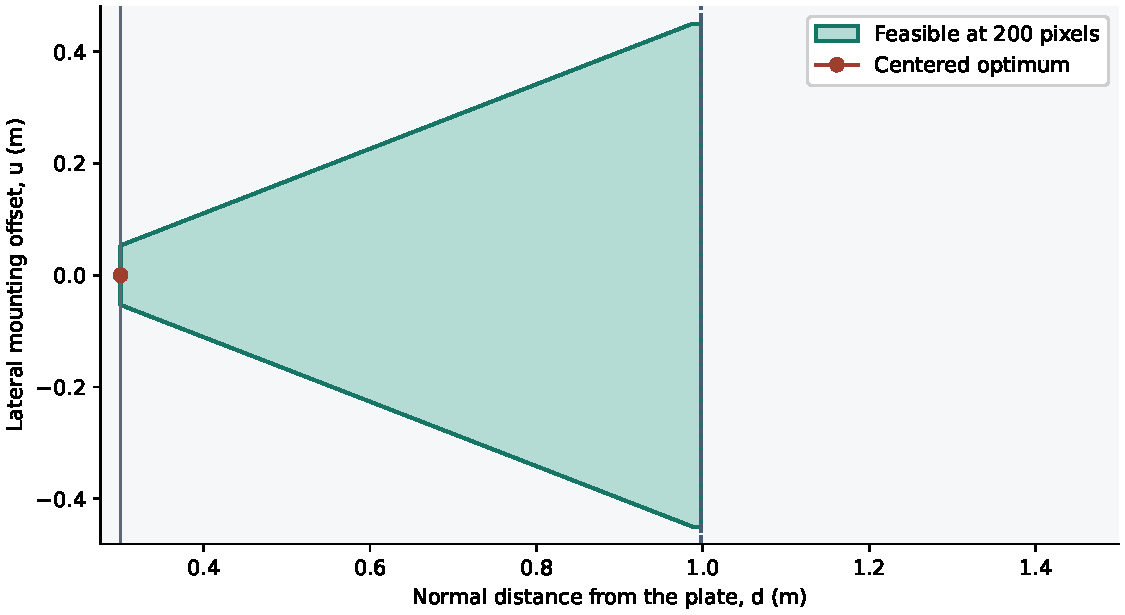
\includegraphics[width=.75\linewidth,height=.23\textheight,keepaspectratio]{label_region.pdf}
\caption{Accepted distance and offset settings on the fixture.}\label{fig:plate}
\end{figure}
\begin{table}[H]\centering
\caption{Sensitivity to the required image width. Fractions use the full \(1.08\,\mathrm{m}^2\) fixture parameter rectangle.}
\PlateTable
\end{table}
The quality objective is to maximize the projected pixel width \(P(d)\), which decreases strictly with \(d\). At \(d=0.30\) every offset with \(|u|\leq0.053205\) is optimal. Centering at \(u=0\) maximizes the smaller of the two edge clearances and leaves 147.45 pixels per side. The best nominal width is 665.11 pixels. Checking both image edges directly on a \(9600\times6400\) midpoint grid gives areas within \(3.3\times10^{-5}\,\mathrm{m}^2\) of the integral at all three thresholds.

\clearpage
\subsection{Which Setting Survives a Mounting Error?}
The nominal solution commands the camera to its nearest permitted position. A small inward mounting error would put it beyond that stop. Suppose the command is \((d_0,u_0)\) and the physical position can be anywhere within \(d_0\pm e,\ u_0\pm v\). The stated bounds are test values. All combinations inside this box are allowed.

Let \(U=0.45\) and \(D=\min(1.50,960w/(2tP_0))\). A command guarantees the travel limits, both visible label edges and the pixel requirement exactly when
\begin{align}
 e+\max\{0.30,(w/2+v)/t\}\ \leq &\,d_0\leq D-e,\\
 |u_0|\ \leq &\,\min\{U-v,(d_0-e)t-w/2-v\}.
\end{align}
The nearest realization \(d_0-e\) has the narrowest field of view, while the farthest realization \(d_0+e\) gives the fewest pixels. The largest possible offset magnitude is \(|u_0|+v\). These extrema give necessary and sufficient conditions because the error box includes its corners. The same three quantities therefore determine the integral of the feasible lateral width over the commanded distance.

\begin{table}[H]\centering
\caption{Guaranteed performance at the best centred command for equal axial and lateral tolerance. The share uses the original \(1.08\,\mathrm{m}^2\) command rectangle.}
\ToleranceTable
\end{table}
Maximizing the worst-case image width selects the smallest admissible \(d_0\). Centering then maximizes the guaranteed clearance at the nearer image edge. With \(e=v=1\) cm, the commanded 31\,cm delivers physical distances between 30 and 32\,cm. It guarantees 623.54 pixels across the label and 119.73 pixels of clearance at the less favourable edge. The feasible share drops from 32.89\% to 29.97\%.

An independent test projected both label edges at all four box corners on a \(4800\times3200\) grid of commands. The analytic and direct classifications agreed at every tested grid point for each tolerance. This checks the geometry. The 200-pixel criterion is a framing and sampling requirement. Establishing actual readability would require images with known text and measurements of blur and lighting.

\clearpage
\section{Question 2. Measurement and the Initial Queue}
\subsection{Choosing Two Temperature Channels}
Channels A through D read \(22.4,22.7,22.1,22.6^\circ\mathrm C\); their independent repeatability standard deviations are \(0.35,0.45,0.60,0.90^\circ\mathrm C\). Preparing one reading costs \(8,7,4,2\) instrument-minutes respectively. Write \(Y_i=T+B+e_i\), where the reference offset \(B\) has mean zero and standard deviation \(c=0.20^\circ\mathrm C\). All \(e_i\) and \(B\) are independent Gaussian variables, and \(\operatorname{Var}(e_i)=v_i\). The same \(B\) enters both readings.

For selected channels \(i,j\), any linear unbiased estimate has the form \(\hat T=w_iY_i+w_jY_j\) with \(w_i+w_j=1\). Minimizing \(c^2+w_i^2v_i+w_j^2v_j\) subject to that equality gives
\begin{equation}
 w_i=\frac{v_i^{-1}}{v_i^{-1}+v_j^{-1}},\qquad
 V_{ij}=c^2+\frac{1}{v_i^{-1}+v_j^{-1}} .
\end{equation}
The quadratic is strictly convex. The common reference variance persists regardless of the weights. Table~\ref{tab:pairs} evaluates every pair before applying the cost constraint.

\begin{table}[H]\centering
\caption{Pair selection at the 12 instrument-minute budget.}\label{tab:pairs}
\PairTable
\end{table}

The feasible minimum is A+C, with weights \(0.746114\) and \(0.253886\). Their estimate is \(22.32383^\circ\mathrm C\). Using the known Gaussian error scales gives the 95\% interval \(\hat T\pm1.959964\sqrt{V_{AC}}=[21.61337,23.03430]^\circ\mathrm C\). This is uncertainty about the common temperature across repetitions of the stated calibration experiment. An unknown fixed reference bias would instead require a separate calibration correction.

At a budget of 10 the best pair is A+D. Increasing the budget to 12 replaces D with C, and at 15 the more precise A+B pair becomes feasible. Direct inversion of each pair's \(2\times2\) covariance matrix reproduced the weights and variances for all six pairs. The instrument labels in this subsection are independent of the work-order identifiers below.

\clearpage
\subsection{Two Workstations and Five Orders}
One bench processes each record for \(p_j\) minutes. A single reviewer then needs \(q_j\) minutes to sign it off. Waiting space is unlimited. The review desk takes records in bench order. Processing starts as soon as both the job and its station are available. Table~\ref{tab:jobs} also lists the later orders used in Question~4.
\begin{table}[H]\centering
\caption{Constructed service times. New records arrive only in the specified scenarios.}\label{tab:jobs}
\JobsTable
\end{table}
For a permutation \(\pi\), let \(I_i\) and \(C_i\) be the completion times of its \(i\)-th record at the two workstations. Taking \(I_0=C_0=0\) gives
\[
 I_i=I_{i-1}+p_{\pi_i},\qquad
 C_i=\max(I_i,C_{i-1})+q_{\pi_i}.
\]
We minimize \(C_5\). Among tied schedules, we minimize \(\sum_i C_i\) and then use alphabetical order. The comparison policy takes the records in their initial registration order A--B--C--D--E.
\begin{table}[H]\centering
\caption{Initial timelines of the two admissible queues, in minutes.}\label{tab:base}
\BaseTable
\end{table}
The 34 minutes of inspection and the shortest possible final review of 2 minutes imply \(C_5\geq36\). B--C--D--A--E attains 36. Eight of the 120 permutations attain this bound. Registration order takes 39 minutes. Starting B first releases a record to review at minute 3, allowing its ten-minute review to overlap inspection of C. Johnson's two-machine rule independently returns B--D--C--A--E and the same 36-minute optimum \cite{johnson}. Summed completion times are 127 minutes for Johnson's sequence and 124 for the selected tie-break.

\clearpage
\subsection{When Temperature Preparation Uses the Inspection Bench}
The 36-minute baseline covers the five basic records. Consider an additional temperature check on work order A. Assume that the inspection bench is occupied throughout the preparation of both selected channels, and that these minutes occur serially in addition to A's original eleven. This variant links measurement precision to a resource shared with other work. The outage comparisons in Question~4 retain the basic service times.

For pair \(i,j\) with preparation times \(h_i,h_j\), set \(p_A'=11+h_i+h_j\) and keep all other processing times unchanged. Count the two channels' common reference variance in \(V_{ij}\) as before. We minimize the pair \((C_{\max},\sqrt{V_{ij}})\), presenting the choices for which no other pair improves one measure without worsening the other.
\begin{figure}[H]\centering
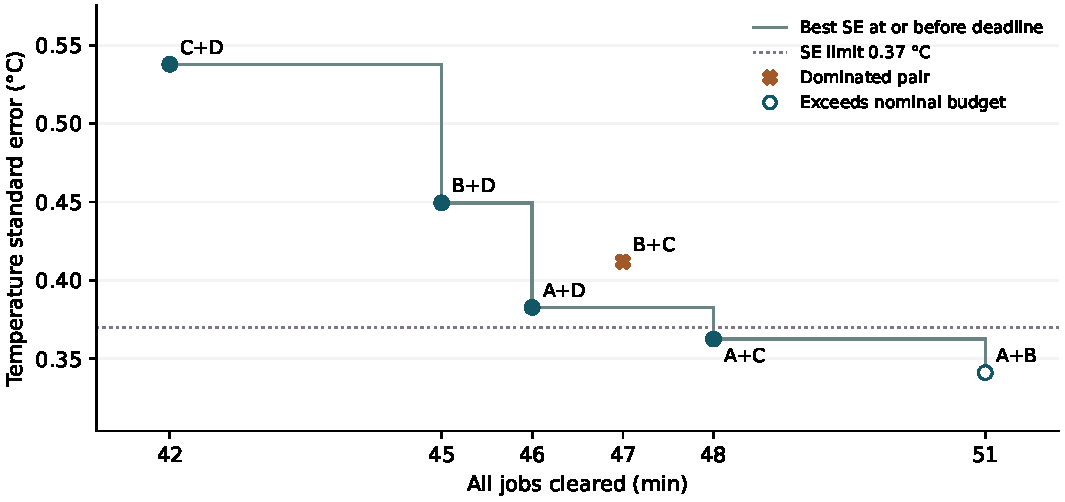
\includegraphics[width=.88\linewidth,height=.30\textheight,keepaspectratio]{joint_frontier.pdf}
\caption{Temperature uncertainty versus the earliest possible clearance of all five records. Only discrete channel pairs are available.}
\end{figure}
All six pairs and all 120 orders per pair were evaluated. For every pair, B--C--D--A--E attains the lower bound \(36+h_i+h_j\). No rearrangement eliminates the added bench work. Five pairs are efficient before imposing the 12-minute instrument budget. B+C is dominated by A+D, which clears in 46 rather than 47 minutes and reduces the standard error from \(0.412\) to \(0.383^\circ\mathrm C\).

Under the 12-minute budget, a 46-minute clearance deadline selects A+D. At 48 minutes A+C becomes feasible and reduces the standard error to \(0.362^\circ\mathrm C\). If the shop requires a standard error of at most \(0.37^\circ\mathrm C\), the first feasible deadline is 48 minutes. The time cost depends on whether preparation actually occupies the bench. Measuring that occupancy would determine which version of the calculation applies.

\clearpage
\section{Question 3. Accuracy of a Fixed-Reference Calibration}
\subsection{A Probability on the Circle}
An instrument views a surveyed reference at distance \(R=40\). After cumulative movement \(s\), its reference-coordinate errors have independent \(N(0,\sigma^2)\) components with \(\sigma=0.30+0.02s\). The independent zero-offset and control errors have standard deviations \(0.8^\circ\) and \(0.6^\circ\). Their sum has standard deviation \(\tau=1^\circ\). Three independent standard normals \(X,Y,Z\) suffice for the distribution of the angular error
\begin{equation}
 D=\operatorname{wrap}_{[-\pi,\pi)}\!\left[
 \operatorname{atan2}(\sigma Y,R+\sigma X)+\tau Z\right].
\end{equation}
Reflection of either coordinate-error component leaves its law unchanged, so the formula also covers the opposite signed-coordinate convention. The requirement is \(p(\sigma)=\Pr(|D|\leq\delta)\geq0.95\), for \(\delta=5^\circ\).

Rotate the noisy reference vector by the instrument angle \(g=\tau z\), conditional on \(Z=z\), and divide by \(\sigma>0\). Isotropy leaves the covariance matrix equal to the identity. The rotated vector has mean \((m,n)=(R/\sigma)(\cos g,\sin g)\). Conditional on an additional standard horizontal residual \(u\), success requires a positive abscissa \(m+u\) and a vertical component between \(-h\) and \(h\), where \(h=(m+u)\tan\delta\). With standard normal density \(\phi\) and distribution \(\Phi\),
\begin{equation}
 p(\sigma)=\int_{\mathbb R}\!\phi(z)
 \int_{-m}^{\infty}\!\phi(u)
 \{\Phi(h-n)-\Phi(-h-n)\}\,du\,dz .
 \label{eq:sector}
\end{equation}
This event is a sector in the plane and handles the angle convention across the cut at \(\pm\pi\).

For uniqueness, couple samples at different scales using the same \(X,Y\). The unsigned positional angle is \(\operatorname{atan2}(|Y|,R/\sigma+X)\), a strictly increasing function of \(\sigma\) almost surely. The centred wrapped-normal density of the independent instrument error decreases with circular distance from zero. This follows from the theta-function product in \cite{theta}. For an even decreasing density \(f\), the mass in an arc centred a distance \(a\) from zero has derivative \(f(a+\delta)-f(a-\delta)\leq0\), with both arguments read on the circle. Thus \(p(\sigma)\) decreases strictly. A crossing of 0.95 identifies the maximum allowed scale.

\clearpage
\subsection{Limit, Independent Simulation and Error Shares}
Integrating equation~\eqref{eq:sector} with 96-point Gauss--Legendre rules and solving for \(p=0.95\) gives
\begin{equation}
 \sigma_* = 1.636745169\,\mathrm m,\qquad
 s_*=(\sigma_*-0.30)/0.02=66.83725843\,\mathrm m .
\end{equation}
At 80\,m, any law \(\sigma(s)=a+bs\) with \(a,b\geq0\) meets the requirement exactly when \(a+80b\leq\sigma_*\). For instance, keeping \(a=0.30\,\mathrm m\) requires \(b\leq(\sigma_*-0.30)/80\simeq0.016709315\). The nominal law gives \(\sigma(80)=1.90\,\mathrm m\). Its hit probability is \(91.5068\%\).

\begin{table}[H]\centering
\caption{Integrated probability and a direct simulation with two million independent trials per setting.}\label{tab:noise}
\NoiseTable
\end{table}
\begin{figure}[H]\centering
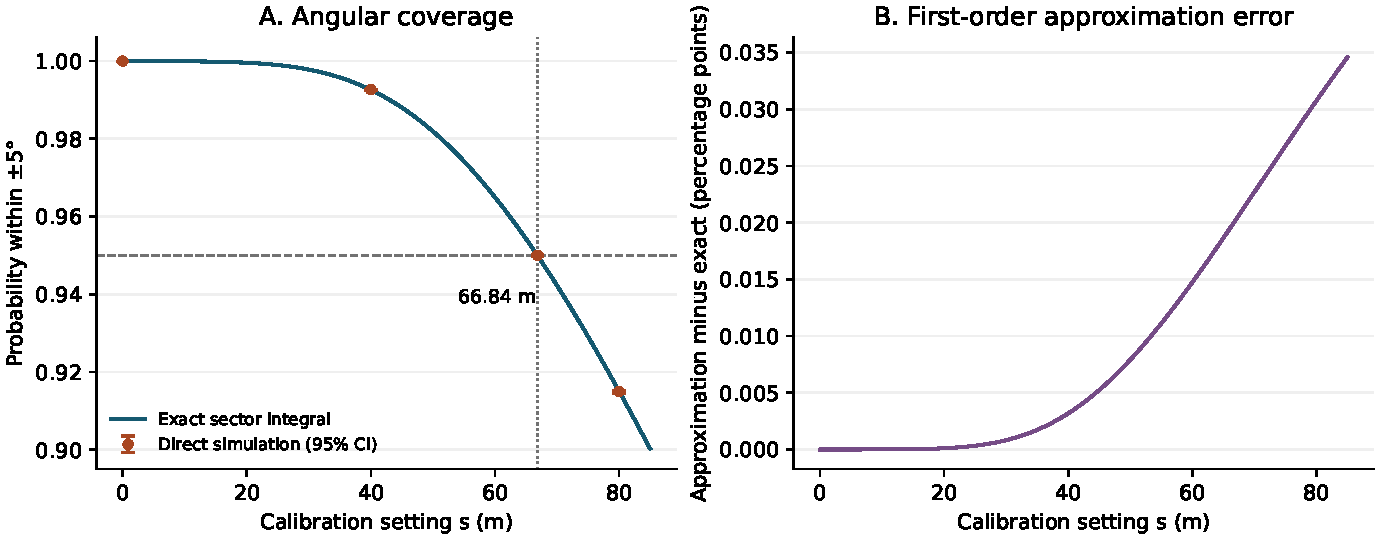
\includegraphics[width=.93\linewidth,height=.25\textheight,keepaspectratio]{q3_validation.pdf}
\caption{Coverage against cumulative movement; the right panel resolves the small linearization error.}\label{fig:noise}
\end{figure}
The simulation draws the two coordinate and two instrument errors, takes \(\operatorname{atan2}\) and wraps the sum directly. Intervals in Table~\ref{tab:noise} are pointwise 95\% Wilson intervals \cite{wilson}. The same random numbers across settings reduce noise in comparisons. Truncating each normal integral at ten standard deviations discards probability at most \(4\Phi(-10)<3.1\times10^{-23}\); orders 64 and 128 agree with the reported root to within \(2\times10^{-13}\,\mathrm m\).

Linearizing at the nominal reference gives \(V_D\approx(\sigma/R)^2+\tau^2\) in radians squared. Its distance limit, 66.92230\,m, exceeds the exact one by 0.08504\,m. At the boundary, coordinate error accounts for 84.61\% of the linearized variance, zero offset for 9.85\% and control error for 5.54\%. The 64-to-36 split applies within the instrument contribution alone. Reducing coordinate drift therefore has the largest first-order leverage near this case's threshold.

\clearpage
\section{Question 4. Changes to the Maintenance Queue}
\subsection{What Can Change at Minute Eight}
Both policies begin with B--C--D--A--E. At minute 8 a notice reveals any new work and its service requirements, and specifies when a planned desk closure will end. No further event occurs. Inspection of B and C has already started. Those positions are frozen. Any review interrupted by a closure resumes first with its residual work. Jobs completing exactly at minute 36 count as on time.

The keep policy appends new work to the initial sequence. The alternative enumerates every permutation of the unfrozen suffix, including keep. Changing the suffix occupies the inspection bench for two minutes when it next becomes free, from minute 12 to 14 in this case. The review desk can continue its own work during that changeover. A retained sequence incurs no changeover.

For each admissible order the program applies the two-stage recurrence, splitting a review into two intervals if it crosses an outage. Let \(k=\#\{j:C_j\leq36\}\) and let \(N\) count all announced records. We rank schedules by decreasing \(k/N\), then increasing actual clearance time \(C_{\max}\). Among equal scores the search first prefers retaining the queue, then minimizes summed completion times and uses the job identifiers. We also record a capped last time of 36 when a job misses the window. Actual clearance separates late-finishing schedules with the same capped score.
\begin{table}[H]\centering
\caption{Matched scenarios. The count and clearance time measure different consequences of a queue change.}\label{tab:events}
\ScenarioTable
\end{table}
S0 is the control. S1 adds F. S2 closes the desk for 8 minutes. S3 combines S1 and S2. S4 adds F and G together, and S5 combines those two arrivals with a 12-minute closure. They test arrivals alone, capacity loss alone and their interaction. No occurrence probabilities are assumed.

\clearpage
\subsection{When Changing the Queue Pays}
\begin{figure}[H]\centering
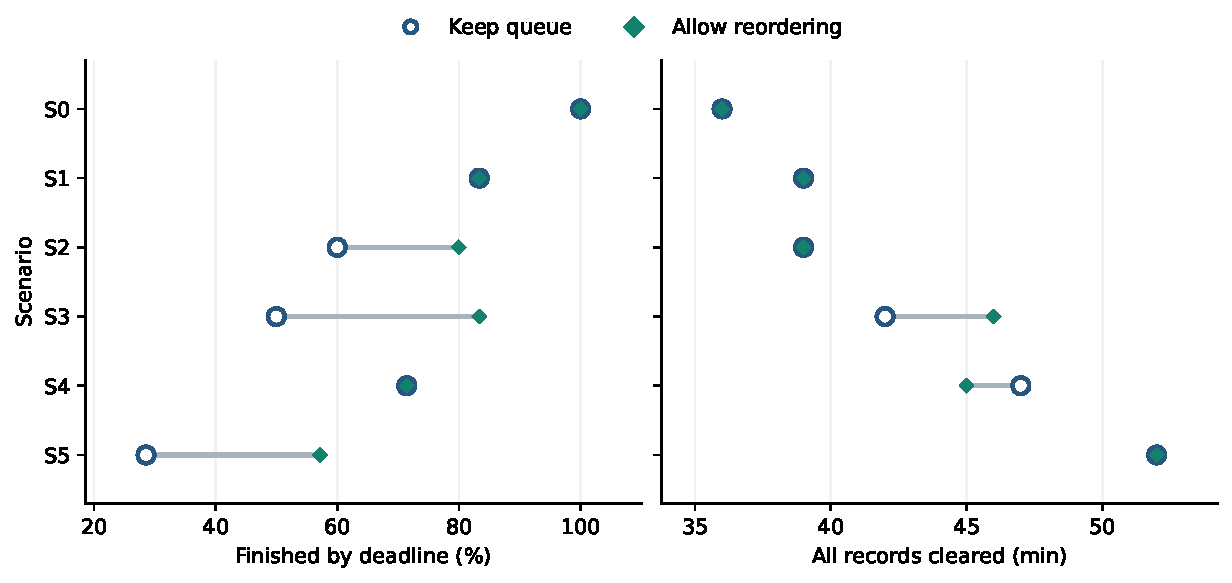
\includegraphics[width=.94\linewidth,height=.32\textheight,keepaspectratio]{schedule_comparison.pdf}
\caption{Policy comparison across six events. Higher completion fractions and shorter clearance times are preferable.}\label{fig:schedule}
\end{figure}
S0 and S1 retain the original queue. In S2, moving E earlier increases the number finished by the deadline from three to four without changing final clearance. In S3 the revised suffix brings both short records E and F forward. Five jobs finish on time, compared with three under keep, while clearance grows from 42 to 46 minutes. This is a choice a manager could reverse by changing the objective.

S4 illustrates the second scoring criterion: each policy completes five of seven on time, but reordering shortens the tail from 47 to 45 minutes. In S5, four of seven finish on time under reordering and two under keep; both clear at minute 52. Allowing reordering can never worsen the specified lexicographic score because keeping the queue is a candidate with its actual cost. 

\noindent\textbf{Sensitivity to queue-update time.} \SensitivityText

\noindent\textbf{Checks.} The six suffix searches visit 6, 24, 6, 24, 120 and 120 candidates. A minute-by-minute replay checks remaining work and station occupancy against the event calculation for each candidate. The appendix lists both realized timelines for every scenario. These comparisons assume the notice gives the correct recovery time.

\clearpage
\subsection{Choosing Before the Repair Duration Is Known}
At minute 8, suppose the shop knows which orders arrived and that the desk has closed. The shop must pick one remaining queue before learning the duration \(L\) of the repair. The committed B--C prefix, two-minute changeover, 36-minute deadline and service times remain the same. To study the value of knowing \(L\), assign equal probability to the thirteen integer durations from 4 through 16 minutes. This is a specified stress experiment with no fitted failure data.

Write \(k(\pi,\ell)\) for the number on time and \(C(\pi,\ell)\) for the actual clearance of queue \(\pi\) when \(L=\ell\). For a fixed set of new orders, choose the same \(\pi\) for every duration. For probability weights \(w_\ell\), the objective is
\[
 \mathop{\mathrm{lex\,min}}_{\pi}\left(
  -\sum_{\ell=4}^{16} w_\ell k(\pi,\ell),\
   \sum_{\ell=4}^{16} w_\ell C(\pi,\ell)\right).
\]
We first minimize the negative expected count, then minimize expected clearance among count-optimal queues. We compare retention, sorting the remaining orders by their total service time, optimizing for the mean duration, and optimizing these two expectations. A perfect-information benchmark selects a separate best queue for each realized duration. Every method pays the same changeover cost when it reorders.

\begin{table}[H]\centering
\caption{One new order F. Expectations over the thirteen equally weighted repair durations.}
\RecoveryTable
\end{table}
For F, the distribution-based and mean-duration rules select the same queue. Knowing the duration in advance brings no additional on-time orders on average, but would clear the work 1.15 minutes earlier than the fixed decision. With a desk closure and \emph{no} new order, the comparison changes: the distribution-based decision completes \(49/13=3.769\) orders on time, compared with \(48/13=3.692\) for the mean-duration rule. Optimizing for a mean input can therefore miss the best queue even when all expected service times are known.

\clearpage
\subsection{Which Durations Justify the Change?}
\begin{figure}[H]\centering
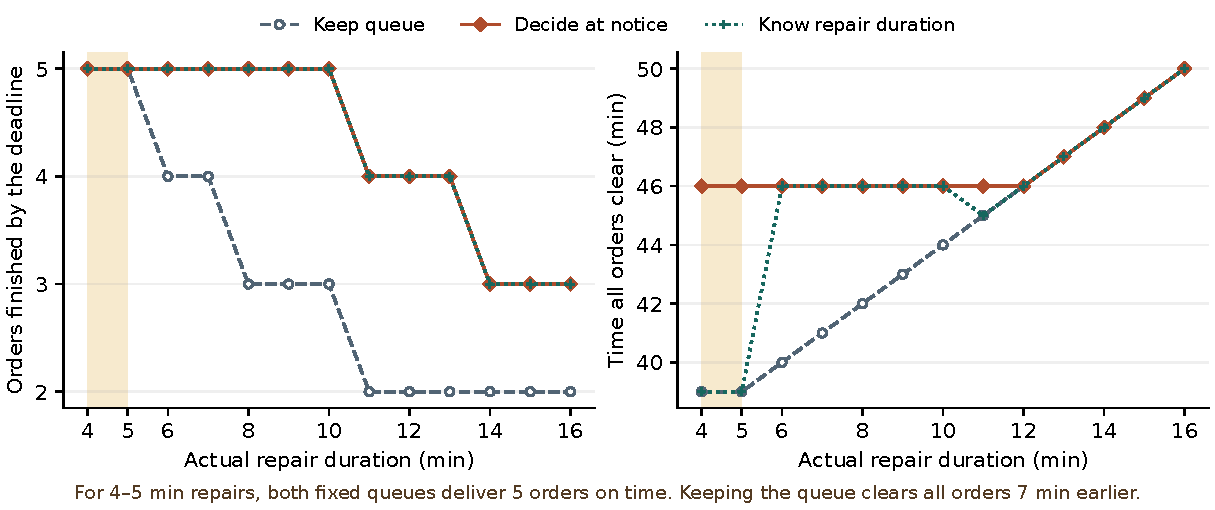
\includegraphics[width=.94\linewidth,height=.30\textheight,keepaspectratio]{uncertain_recovery.pdf}
\caption{One new order F. Both fixed queues are chosen at notice. The perfect-information benchmark knows the repair duration in advance.}\label{fig:repair}
\end{figure}
In Figure~\ref{fig:repair}, queue B--C--E--F--A--D gains exactly two on-time records over keeping the queue for six of the thirteen durations, namely 8 through 13 minutes. For four- and five-minute repairs both queues finish five on time, but keeping clears at minute 39 versus minute 46. At the other five durations the revised queue gains one on-time record. These observations explain both the mean improvement of \(17/13=1.31\) on-time records and the added mean clearance time of \(35/13=2.69\) minutes.

Let \(v\ge0\) be the clearance delay the shop would accept for one extra on-time order. For each of the 24 feasible queues, minimize its cost \(\mathbb E[C]-v\mathbb E[k]\) against all competitors. Each cost is a line in \(v\). Summing clearance times and timely counts over the 13 durations gives integer coefficients for \(13\) times the cost, giving the exact switching values in Table~\ref{tab:value}.
\begin{table}[H]\centering
\caption{Lowest-cost queues for one new order and uniform repair durations. At each switching value, both adjacent queues are optimal.}\label{tab:value}
\small\begin{tabular}{@{}lcrr@{}}\toprule
Delay value \(v\) (min/order) & Queue & \(\mathbb E[k]\) & \(\mathbb E[C]\) (min)\\\midrule
\TradeoffRows
\bottomrule\end{tabular}
\end{table}
Moving from BCDAEF to BCEFDA delays clearance by \(5/13\) minute and gains \(12/13\) on-time order on average. The trade is worthwhile above \(v=5/12\). Moving on to BCEFAD costs another \(30/13\) minutes for \(5/13\) more orders, giving the second switch at \(v=6\). At \(v=35/17\), the first and last queues tie with each other while the middle queue has strictly lower cost.

For the deadline-first objective, we reweight the same durations with weights proportional to \(17-\ell\) or \(\ell-3\), giving mean durations of 8 or 12 minutes. The nominal queue for F remains optimal in these two tests. Its expected on-time count ranges from 3.91 under the long-repair weights to 4.70 under the short-repair weights. The shorter- and longer-repair profiles are alternative assumptions about the same support. Across three arrival batches, we checked all \(13(6+24+120)=1950\) queue--duration pairs against a minute-step replay.

\clearpage
\section{Conclusion}
The recommended settings depend on what the shop can control. A 1\,cm mounting tolerance moves the best camera command to 31\,cm. A two-minute extension of the bench deadline permits the more precise A+C channels in place of A+D. For one order arriving during a repair, the best queue depends on the value of timely delivery. Between \(5/12\) and 6 minutes per extra on-time order, the compromise queue brings forward E and F and schedules D before A. It clears only 0.38 minute later than retention while delivering 0.92 more orders on time on average.

The strongest evidence here is conditional: the idealized geometry, Gaussian calibration law, and enumerated schedules yield reproducible decisions under stated inputs. To test them on a shop floor, one would need repeat fixture measurements, images with readable-text reference labels, and time-stamped bench occupancy and repair records. Comparing predicted coverage and policy outcomes on later shifts would directly test assumptions that numerical replay cannot validate.

\begin{thebibliography}{9}
\bibitem{source} ShuWei Cup Organizing Committee. \emph{2026 Autumn Challenge, Problem B}, Question 3, pp.~4--5. Source of the stated angular calibration parameters.
\bibitem{johnson} S. M. Johnson. Optimal two- and three-stage production schedules with setup times included. \emph{Naval Research Logistics Quarterly}, 1, 61--68, 1954. \url{https://doi.org/10.1002/nav.3800010110}.
\bibitem{theta} NIST. \emph{Digital Library of Mathematical Functions}, Sec.~20.5(i), Eq.~20.5.3, Jacobi's triple product. \url{https://dlmf.nist.gov/20.5.E3}.
\bibitem{wilson} NIST/SEMATECH. \emph{e-Handbook of Statistical Methods}, Sec.~7.2.4.1, Confidence Intervals. \url{https://www.itl.nist.gov/div898/handbook/prc/section2/prc241.htm}.
\end{thebibliography}
\subsection*{Computational Record}
The companion archive contains the case inputs, six numerical scripts, the numerical results, figures, table generator and editable manuscript. OpenAI Codex assisted in constructing the practice data, performing the calculations, and writing the report. Running \code{python reproduce.py} regenerates the results and builds the PDF. Running \code{python reproduce.py --verify} verifies the file hashes. The Chinese guide lists the environment and commands.
\clearpage
\section*{Appendix. Workstation Timelines}
\addcontentsline{toc}{section}{Appendix. Workstation Timelines}
Times below are minutes from the initial release. Each row follows a single record through both workstations under each policy. A split review interval identifies the work done before and after a closure. The inspection-bench changeover for a revised queue occupies \([12,14)\) in the cases shown. Gaps between recorded intervals are idle or unavailable periods.
\AuditAppendix
\end{document}
